\input{../Common/commands}

\begin{document}

\graphicspath{ {../Common/images/} }
\input{../Common/map}
\graphicspath{ {images/} }


%----------------------------------------------------------------
% PAGE TITLE
% ----------------------------------------------------------------
\pgclrred
\title{\headerpres{Data Analysis: \\ Text and Network Analysis}}
\author{\vspace{3cm} Institute of Technology Tallaght}
\date{Department of Computing}
\maketitle
\newpage

% ----------------------------------------------------------------
% PAGE Multinomial Bayes
% ----------------------------------------------------------------
\headerch{Multinomial Na\"ive Bayes \\for the Prediction of Document Type}

\begin{itemize}
\item Na\"ive Bayes can be used with unstructured data
\item One example is the \emph{classifiaction of documents}
\item Documents are treated as \emph{bags of words}
\item As in basic Na\"ive Bayes, the key to estimating the probability of a document belonging to a class, given the evidence (i.e. the count of different words in it), are the probabilities of documents having a particular combination of words when they are in a particular class (i.e. the probability of evidence given the outcome). This is calculated as:

  $$P(E|C) = N! \times \prod\limits_{i=1}^k \dfrac{P_i^{n_i}}{n_i!}$$

  where $N = n_1 + n_2 + ... + n_k$ is the number of words in the document being classified, $k$ is the number of unique words in all the documents in the data set (all training documents), $n_1, n_2 ...$ are the counts of each of these unique words in the document that is being classified and $P_i$ is the probability of unique word $i$ appearing across all documents of class $C$ in the training set training set.

\item The probabilities of membership in different classes are then calculated for a document as:

  $$P(C|E) = \dfrac{P(E|C_1)P(C_1)}{P(E|C_1)P(C_1)+P(E|C_2)P(C_2)+..._P(E|C_o)P(C_o)}$$

  where $P(C_i)$ is the \emph{a priori} probability of a document belonging to class $C$ and $o$ is the number of document classes (types).
  
\end{itemize}

\newpage


\headerss{\underline{Example}}

Let's say there are two words in the vocabulary of a group of documents: \bt{yellow} and \bt{blue}. A type of document called 'yellowish green', which we will denote with \bt{Y75\_B25}, has $P(\bt{yellow}|\bt{Y75\_B25})=0.75$ and $P(\bt{blue}|\bt{Y75\_B25})=0.25$. The probability of a 'yellowish green' document consisting of the words \bt{\{yellow, yellow, yellow\}} is:
$$ P(\bt{yellow, yellow, yellow}|\bt{Y75\_B25})=3! \times \dfrac{0.75^3}{3!} \times \dfrac{0.25^0}{0!}= 0.42$$
Now let's say that there is only one other class, 'very blue green', which we will denote with \bt{Y10\_B90} and which has $P(\bt{yellow}|\bt{Y10\_B90})=0.1$ and $P(\bt{blue}|\bt{Y10\_B90})=0.9$. The probability of a 'very blue green' document consisting of the words \bt{\{yellow, yellow, yellow\}} is:
$$ P(\bt{yellow, yellow, yellow}|\bt{Y10\_B90})=3! \times \dfrac{0.1^3}{3!} \times \dfrac{0.9^0}{0!}= 0.001$$
We can see that the prior probabiliy of class \bt{Y10\_B90} would have to be about 250 or more times greater than that of class \bt{Y75\_B25} in order for a classification of the given document as \bt{Y10\_B90} to happen.


\newpage
\headerch{Importance of Nodes and Page Rank}

\begin{itemize}
\item When network connections are directional, node influence or rank can be calculated
\item One way to do this is using a link analysis algorithm, such as the Google Page Rank algorithm. With this The algorithm is based around the idea that the more in-links a node has, the more influential it is considered to be.
\item The model will be presented using an example:

  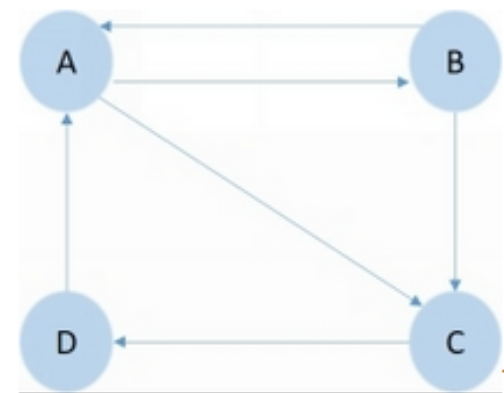
\includegraphics[width=0.4\textwidth]{nodes.png}

  For the four nodes in the picture, the values of influence (or rank) are related as follows:
\begin{flalign*}
  &Ra = 0.5Rb + Rd\\
  &Rb = 0.5Ra\\
  &Rc = 0.5Ra + 0.5Rb\\
  &Rd = Rc
\end{flalign*}

  The \emph{influence matrix} is:

  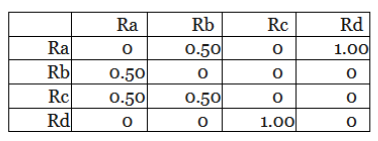
\includegraphics[width=0.4\textwidth]{influence_matrix.png}

  \newpage
  Before calculation starts, equal rank is assigned to all the nodes, after which they have the following values:

  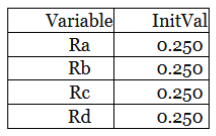
\includegraphics[width=0.2\textwidth]{init.png}

  Then an iterative process of assigning new rank values is performed, using the values from the previous iteration as the right-hand-side values in the equations.
  
  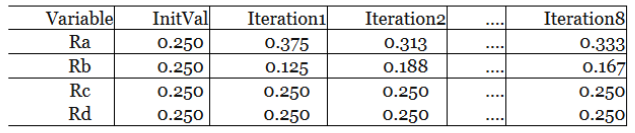
\includegraphics[width=0.6\textwidth]{it3.png}

  The process is stopped once the rank values stabilise.

  \newpage

  The Google Page Rank algorithm also includes a \emph{damping factor} accounting for the fact that some proportion of page requests do not come from another page:

\begin{flalign*}
  &Ra = \dfrac{1-d}{N} + d\times(0.5Rb + Rd)\\
  &Rb = \dfrac{1-d}{N} + d\times(0.5Ra)\\
  &Rc = \dfrac{1-d}{N} + d\times(0.5Ra + 0.5Rb)\\
  &Rd = \dfrac{1-d}{N} + d\times(Rc)
\end{flalign*}

Typically, $d=0.85$. This number represents the frequency with which the average web-surfer accesses pages from bookmarks rather than by link from another page.
  
   
\end{itemize}





\newpage
%----------------------------------------------------------------
% PAGE REFERENCES
% ----------------------------------------------------------------
\headersec{References}

\textbf{[DSB]} \emph{Data Mining: Practical Machine Learning Tools and Techniques}, by Ian H. Witten, Eibe Frank, Mark A. Hall, Christopher J. Pal, Kindle Direct Publishing eBook, 2016.

\textbf{[MSD]} \emph{Making Sense of Data I: A Practical Guide to Exploratory Data Analysis and Data Mining}, by Glenn J. Myatt and Wayne P. Johnson, John Wiley \& Sons, 2014. 


\end{document}

